% !TEX program = pdflatex
\documentclass[aspectratio=169,11pt]{beamer}

\usetheme{Madrid}
\usecolortheme{whale}
\usefonttheme{structurebold}
\setbeamertemplate{navigation symbols}{}
\setbeamertemplate{footline}[frame number]

% Beamer-safe preamble (no enumitem / geometry / fancyhdr)
\usepackage{graphicx}
\usepackage{booktabs}
\usepackage{amsmath,amssymb}
\usepackage{listings}
\usepackage{xcolor}
\usepackage{tikz}
\usetikzlibrary{arrows.meta,positioning,shapes.geometric}
\usepackage{pgfplots}
\pgfplotsset{compat=1.18}

\definecolor{codebg}{RGB}{248,248,248}
\definecolor{codeframe}{RGB}{220,220,220}
\lstdefinestyle{projectstyle}{
  backgroundcolor=\color{codebg},
  basicstyle=\ttfamily\small,
  breaklines=true,
  frame=single,
  rulecolor=\color{codeframe},
  showstringspaces=false,
  tabsize=2
}
\lstset{style=projectstyle}

\definecolor{routeblue}{RGB}{66,133,244}
\definecolor{routegreen}{RGB}{52,168,83}
\definecolor{routeorange}{RGB}{251,188,5}
\definecolor{routegray}{RGB}{95,99,104}


\title[Semantic Search for Nepali Law]{Semantic Search for Nepali Municipal Legal Documents}
\subtitle{Hybrid PDF Extraction, Chunking, and Retrieval Evaluation}
\author{Student Research Presentation}
\institute{Department of Computer Science}
\date{Six-Minute Beamer Presentation}

\begin{document}

%--------------------------------------------------
\begin{frame}
  \titlepage
\end{frame}

%--------------------------------------------------
\begin{frame}{Outline}
  \tableofcontents
\end{frame}

%--------------------------------------------------
\section{Background}
\begin{frame}{Background and Motivation}
  \begin{itemize}
    \item Kathmandu Valley laws are published across municipal websites as PDF files.
    \item The collection includes national laws, municipal bylaws, procedures, and financial acts.
    \item Many users need simple procedural answers, but keyword search across PDFs is weak.
    \item A retrieval system must first extract reliable Nepali text, split it into useful chunks, and evaluate whether search returns the right legal section.
  \end{itemize}
\end{frame}

%--------------------------------------------------
\section{Aim}
\begin{frame}{Aim and Objectives}
  \begin{block}{Aim}
    Build and evaluate a small retrieval-ready corpus for Nepali municipal legal documents.
  \end{block}
  \begin{enumerate}
    \item Scrape and curate a focused corpus of legal PDFs.
    \item Route text-based PDFs and scanned PDFs through suitable extractors.
    \item Convert extracted text into semantic chunks.
    \item Benchmark dense retrieval using query-level ground truth.
    \item Identify practical errors that affect retrieval quality.
  \end{enumerate}
\end{frame}

%--------------------------------------------------
\section{Literature}
\begin{frame}{Literature Review}
  \begin{itemize}
    \item Legal information retrieval requires high precision because answers depend on exact sections and conditions.
    \item Retrieval-augmented generation depends on document preprocessing: extraction quality and chunk boundaries directly affect final answers.
    \item Multilingual embedding models are usually stronger for Nepali and code-switched queries than English-only baselines.
    \item Prior OCR work shows that scanned Devanagari documents need separate quality tracking because recognition errors become retrieval errors.
  \end{itemize}
\end{frame}

%--------------------------------------------------
\section{Methods}
\begin{frame}{Method: End-to-End Pipeline}
  \centering
  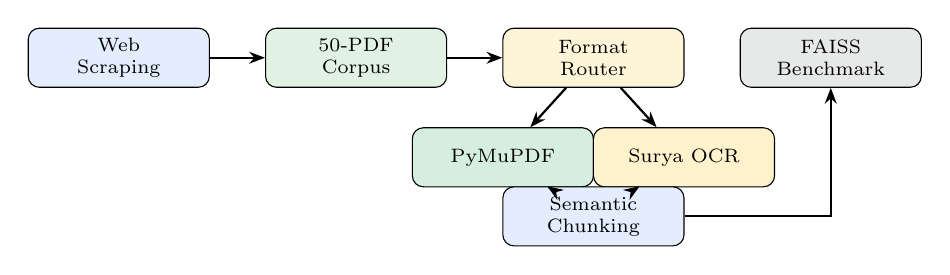
\begin{tikzpicture}[
    node distance=0.5cm and 0.7cm,
    box/.style={draw, rounded corners, align=center, minimum width=2.3cm, minimum height=0.75cm, font=\scriptsize},
    arrow/.style={-{Stealth[length=2mm]}, thick}
  ]
    \node[box, fill=routeblue!15] (scrape) {Web\\Scraping};
    \node[box, fill=routegreen!15, right=of scrape] (curate) {50-PDF\\Corpus};
    \node[box, fill=routeorange!15, right=of curate] (route) {Format\\Router};
    \node[box, fill=routegreen!20, below=of route, xshift=-1.15cm] (text) {PyMuPDF};
    \node[box, fill=routeorange!20, below=of route, xshift=1.15cm] (ocr) {Surya OCR};
    \node[box, fill=routeblue!15, below=1.25cm of route] (chunk) {Semantic\\Chunking};
    \node[box, fill=routegray!15, right=of route] (eval) {FAISS\\Benchmark};

    \draw[arrow] (scrape) -- (curate);
    \draw[arrow] (curate) -- (route);
    \draw[arrow] (route) -- (text);
    \draw[arrow] (route) -- (ocr);
    \draw[arrow] (text) -- (chunk);
    \draw[arrow] (ocr) -- (chunk);
    \draw[arrow] (chunk) -| (eval);
  \end{tikzpicture}
  \vspace{0.3cm}

  \small The pipeline produces raw text, JSONL chunks, extraction summaries, and retrieval metrics.
\end{frame}

%--------------------------------------------------
\begin{frame}{Corpus and Extraction}
  \begin{columns}[T]
    \column{0.48\textwidth}
    \textbf{Curated corpus}
    \begin{itemize}
      \item 50 legal PDFs
      \item 830 total pages
      \item Kathmandu, Lalitpur, Bhaktapur, and federal sources
      \item 45 text-based, 5 scanned
    \end{itemize}
    \column{0.48\textwidth}
    \textbf{Current outputs}
    \begin{itemize}
      \item 50 chunk files
      \item 446 total chunks
      \item 11 evaluation queries
      \item MiniLM baseline CSV generated
    \end{itemize}
  \end{columns}
\end{frame}

%--------------------------------------------------
\section{Evaluation}
\begin{frame}{Evaluation Method}
  \begin{itemize}
    \item Each query has a target legal chunk as ground truth.
    \item Retrieval is evaluated with \textbf{Recall@5} and \textbf{MRR}.
    \item FAISS performs cosine-similarity search over embedding vectors.
    \item Baseline model: \texttt{sentence-transformers/all-MiniLM-L6-v2}.
    \item Multilingual model planned: \texttt{BAAI/bge-m3}.
  \end{itemize}
  \vspace{0.3cm}
  \begin{block}{Why this matters}
    If the correct section is not retrieved, a later RAG answer cannot cite the right legal basis.
  \end{block}
\end{frame}

%--------------------------------------------------
\section{Results}
\begin{frame}{Results and Findings}
  \begin{table}
    \centering
    \begin{tabular}{@{}lcc@{}}
      \toprule
      \textbf{Run} & \textbf{Recall@5} & \textbf{MRR} \\
      \midrule
      MiniLM baseline, 11 queries & 0.000 & 0.000 \\
      BGE-M3 multilingual run & Pending & Pending \\
      \bottomrule
    \end{tabular}
  \end{table}
  \vspace{0.25cm}
  \begin{itemize}
    \item The baseline result is not a final failure of the idea; it reveals evaluation and language mismatch.
    \item Ground-truth chunk IDs required mapping before fair comparison.
    \item Some scanned documents produce sparse chunks, showing OCR quality is a retrieval risk.
  \end{itemize}
\end{frame}

%--------------------------------------------------
\section{Paper Outline}
\begin{frame}{Paper Outline}
  \begin{enumerate}
    \item Introduction: problem, motivation, and objectives.
    \item Related Work: legal retrieval, RAG preprocessing, multilingual embeddings, OCR.
    \item Methodology: scraping, curation, extraction routing, chunking, and benchmarking.
    \item Corpus: sources, document categories, format types, and limitations.
    \item Evaluation: query bank, metrics, and ground-truth alignment.
    \item Results and Discussion: baseline behavior, errors, and improvements.
    \item Conclusion: contributions and future work.
  \end{enumerate}
\end{frame}

%--------------------------------------------------
\section{Conclusion}
\begin{frame}{Conclusion}
  \begin{itemize}
    \item The project builds a working retrieval-preparation pipeline for Nepali municipal legal PDFs.
    \item The strongest contribution is the complete path from scraped PDFs to chunked corpus and benchmarkable queries.
    \item The main lesson is that extraction quality, chunk IDs, and multilingual model choice are as important as the search algorithm.
    \item Next steps: complete OCR validation, run BGE-M3 fully, expand human-labeled queries, and test hybrid BM25 plus dense retrieval.
  \end{itemize}
\end{frame}

%--------------------------------------------------
\begin{frame}{Thank You}
  \centering
  \Huge Questions?

  \vspace{0.8cm}
  \normalsize
  Repository: \texttt{scrapktm}\\
  Slides built with Beamer
\end{frame}

\end{document}
